%%%%%%%%%%%%%%%%%%%% book.tex %%%%%%%%%%%%%%%%%%%%%%%%%%%%%
%
% sample root file for the chapters of your "monograph"
%
% Use this file as a template for your own input.
%
%%%%%%%%%%%%%%%% Springer-Verlag %%%%%%%%%%%%%%%%%%%%%%%%%%


% RECOMMENDED %%%%%%%%%%%%%%%%%%%%%%%%%%%%%%%%%%%%%%%%%%%%%%%%%%%
\documentclass[graybox,envcountchap,sectrefs]{svmono}

% choose options for [] as required from the list
% in the Reference Guide

%\usepackage{mathptmx}
%\usepackage{helvet}
%\usepackage{courier}
%
\usepackage{type1cm}         

\usepackage{makeidx}         % allows index generation
\usepackage{graphicx}        % standard LaTeX graphics tool
                             % when including figure files
\usepackage{multicol}        % used for the two-column index
\usepackage[bottom]{footmisc}% places footnotes at page bottom

\usepackage{newtxtext}       % 
\usepackage[varvw]{newtxmath}       % selects Times Roman as basic font

\usepackage[most]{tcolorbox}

\usepackage{soul} % strike through text

\usepackage{hyperref} % interactive contents

\usepackage[section]{placeins} % floatbarrier

\usepackage{alltt}

\usepackage{svg} % svg images. Doesn't work yet!

\usepackage{caption}


\setcounter{secnumdepth}{0}

\newcommand{\code}[1]{{\fontfamily{cmtt}\selectfont \color{gray} #1}}


% see the list of further useful packages
% in the Reference Guide

\makeindex             % used for the subject index
                       % please use the style svind.ist with
                       % your makeindex program

%%%%%%%%%%%%%%%%%%%%%%%%%%%%%%%%%%%%%%%%%%%%%%%%%%%%%%%%%%%%%%%%%%%%%

\begin{document}

\captionsetup[figure]{labelfont={bf}, labelformat={default}, name={Figure}}

\author{Marco Gähler}
\title{Legacy Code Made Easy}
\subtitle{}
\maketitle

\frontmatter%%%%%%%%%%%%%%%%%%%%%%%%%%%%%%%%%%%%%%%%%%%%%%%%%%%%%%

%\include{foreword}

\tableofcontents

\hypersetup{
    colorlinks,
    citecolor=black,
    filecolor=black,
    linkcolor=black,
    urlcolor=black
}

%\include{acronym}


\mainmatter%%%%%%%%%%%%%%%%%%%%%%%%%%%%%%%%%%%%%%%%%%%%%%%%%%%%%%%

Foreword

This book is based on Michael Feathers book "Working Effectively with Legacy Code" (WELC). It covers a very important topic: how to deal with old, badly structured, untested code. In short, legacy code. Legacy code is a very common problem. Even if you try to write good code to begin with, code tends to rot and becomes legacy code over time. This code is worth trillions and countless teams of software engineers have only one task: to keep this code alive at all costs.

Many of the techniques explained in the afore mentioned book are still useful, but there are certainly some aspects that could be written differently. At times it took me too long to understand certain explanations. A common example is dependency injection (DI), which is now a very common technique to handle complexity. Feathers calls this "parametrize constructor" and in my opinion he doesn't give this technique enough credit. Furthermore, Feathers praises the advantages of object-oriented (OO) code and uses inheritance extensively, which in my opinion is somewhat misguided. Even if he gives some explanation under which conditions inheritance should be used, I think it's easier not to use inheritance at all. Inheritance is brittle and brittle code is bad by definition. In my opinion, even the use of classes should be reduced to a minimum. As I explained in my book "Software Engineering Made Easy", procedural code can do anything that OO code can do as well, and in most cases it's even simpler. 

Now I will use classes and in some cases even inheritance for explaining the concepts. You are working with legacy code afterall and you can't expect your code to become perfect overnight. You have to take small steps that improve your code and if using inheritance is the easiest way to do so, then go ahead. But if you have a choice, I recommend using other techniques that don't involve inheritance.

Another issue is that the book focuses too much on C++ and its particularities like preprocessor macros and linking of custom files. Now this is certainly a book about working with old code and such techniques therefore can be useful, but they shouldn't be first class citizens. Such techniques are desperate measures for special issues and should only be used when absolutely needed.

It also has to be said that WELC nor this book contain solutions for all different kinds of problems. For some specific issues we can give you blueprints on how to solve them, but the main task still lies with the programmer, you.  

As a summary, one can say that WELC stood the test of time, but it deserves a complete overhaul and I decided to skim it down to the very basics. I hope that this overhaul will be read for another twenty years as well.

Marco Gähler

\chapter{Working with Legacy Code}

Don't we all dream of our perfect software project? With a clear architecture and tidy code? Unfortunately in most cases, this is not the reality. Most of us work on old legacy code with little to no apparent structure and certainly no unit tests. This is the reality of software development. The code out there works and is worth trillions. It is not going to be rewritten anytime soon.

Now let's imagine what happens if you suggest to rewrite the code and you miraculously get the approval of your CEO. You may start from scratch. You may do everything right this time. But the first problem is, that your customers still expect some new features. So you can't use the entire software team to write the new code. Instead you can only use a fraction of the team to do the rewrite. Robert C. Martin called this the "Tiger Team"\footnote{Clean Code, Robert C. Martin}. Furthermore, the new software needs to have at least as many features as the old one. Otherwise the customers will refuse to use it. So the Tiger Team has to keep up with the legacy code team in addition to writing the new code. The Tiger Team hast to catch up with the legacy code team which in turn makes progress as well.

Now chances are, that the Tiger Team will never catch up. The once perfect plan didn't work out and the code turned out to be just as bad as the old one. Furthermore, the whole process of rewriting the code may already last several years and the original Tiger Team has long dissolved by now. There are new members in the Tiger Team and they don't know any better how to structure the code than the legacy code team. At some point the CEO will pull the plug and the project of the Tiger Team will be abandoned, while the legacy code still exists.

Of course, this is a very pessimistic scenario. In most cases, at least some parts of the new code can be incorporated into the old code. But a complete rewrite carries an existential risk. It has to be well planed and the risk has to be estimated correctly. In most cases, it makes sense to break the existing code into pieces and rewrite them one by one. This is the topic of this book.

\chapter{Testing}

\textsl{"To me, legacy code is simply code without tests."}

%\raggedleft{ -- Michael Feathers}

\section{Unit Tests}\label{chap:unittests}

If you never wrote any unit tests, you should probably learn it with my other book "Software Engineering Made Easy". I will only give a very short introduction here on the most relevant aspects for this book.

As we'll see many times throughout this book, having good (automated) test coverage with unit tests is paramount. The unit tests serve as a safety net when you perform changes to the code. Unit tests immediately give you feedback whether the code still works as expected. As long as the code you're working with is covered with tests, you can be fairly sure that you didn't break anything. Unit tests can never guarantee that everything works. Edsger Dijkstra tried to make proofs that code works exactly as specified 70 years ago and he failed terribly. Nevertheless, unit tests are by far the best safety net available in software engineering and certainly worth the effort.

Unit tests have three properties:
\begin{itemize}
    \item Unit tests are fast. One test should take only a few milliseconds.
    \item Unit tests are deterministic. They should always return the same result.
    \item Unit tests return only two possible results: pass or fail.
\end{itemize}

This implies that anything which communicates with the outside world, like reading a file, talking to a database or communicating over a network, should be abstracted away and not tested with unit tests. Connections and access to the filesystem should be tested with integration tests, as explained in Software Engineering Made Easy\footnote{Software Engineering Made Easy, Marco Gähler}.

Ultimately, unit tests are also just code. And as with normal code, there are some best practices that you should follow. When in doubt, follow the normal best practices for writing good code. Though there are some differences:
\begin{itemize}
    \item Unit tests have to be really easy to understand. If you don't manage to make them really easy to understand, your code has some real issues.
    \item Unit tests test objects only with their external interfaces. You should never test internal methods of an object. If you have to do so, your object is too complex and you should split it into smaller objects.
    \item Write normal code. No preprocessor macros, no global variables, no black magic. Normal code is the best code.
    \item If a test fails, you shoud know immediately what the problem is. If required, you can have a test name which is a complete sentence. You won't use this name anywhere else, so it doesn't matter that it's so long.
    \item Tests should be as independent of each other as possible. If some code breaks, only the corresponding test should fail. With unit tests, this is generally not a big deal, but once you write integration tests, you really have to make sure that each test is responsible for only one thing.
\end{itemize}

As a rule of thumb, one can say that unit tests can only be written for good code. Of course, there might be exceptions, but those are very rare. Vice versa, if you manage to write unit tests to your code, your code is quite certainly well written.

For these reasons, one can say that unit tests are probably the single most important factor of writing good code. Not only because they facilitate refactoring, but also because they force you to write good code.

Now I assume that you already know how to write unit tests and what they are generally about. So I'll refrain from writing an introduction on unit tests here. 

\section{Test Dirven Development}\label{chap:tdd}

Test Driven Development (TDD) is a very common technique to write good code. The idea is that you write the tests before you write the code. TDD forces you to write good code because you write the tests from a user perspective. Thus, you define how the interface of the code should look like if you had a choice. And it turns out that you always have a choice, you just didn't know so far.

Now, I have to admit that doing TDD is something odd to start with. You should first get used to write proper unit tests before you start with TDD. Though once you got used to it, doing TDD feels actually quite natural. The most important thing is that you need to know what the code is supposed to do exactly. Which is anyway a prerequisite for writing good code.

I highly recommend doing TDD once you are used to it. It certainly improves the quality of your code and there are no downsides to it.

TODO Programming by Difference?

\chapter{Problematic Code}

The goal of this book is quite simple: explain to you how to make your existing code better. This requires two steps: you have to find out why your code is bad, and you need to have an idea how the code could look like instead. There are dedicated books on this topic and I highly recommend you'd read my book "Software Engineering Made Easy"\footnote{Software Engineering Make Easy, Marco Gähler} before you read this book. I will always give some explanations on the code examples here, on why they are bad and how it could be improved, but you should be able to judge these things by yourself. I'm only giving you a very short overview on the most important points.

Here is a list with some signs of bad code. This list is by no means exhaustive, but I think it covers the most common issues.

\begin{itemize}
    \item Classes and functions are too long.
    \item There are too many levels of indentation.
    \item There are no unit tests.
    \item Use of comments instead of good names for variables and functions.
    \item There are no interfaces.
    \item There are global variables.
    \item Functions have too many arguments.
    \item Variables are redefined.
    \item Implementation inheritance is used.
\end{itemize}

\section{Classes and Functions are Too Long}

Classes and functions which are too long share the same problems. They tend to grow over time and start becoming one big unreadable pile of code. I'm not even going to show you an example as it would be a waste of paper. You quite certainly know by now that a function of more than 20 lines of code is generally extremely hard to comprehend. Of course, there are huge differences between functions. Some are 5 lines long and cannot be understood while others are 20 lines long and you still feel perfectly fine. But I hope you get the memo: long functions are pretty hard to understand and should therefore be avoided. The very same argumentation also holds for classes.

There are several indicator whether a function or a class is well written. The simplest and most universally applicable rule is whether you can write a unit test for it. This is a quite good rule of thumb. If you are not able to write a unit test, you don't understand the code well enough. A clear sign that it's too complex. It should be broken into pieces.

Another good rule is the Single Responsibility Principle (SRP), which states that every object should do exactly one thing. 

Let me give you a short example. We start with a class \code{car} which has too many responsibilities.

\begin{programcode}{}\label{prog:car}
\begin{verbatim}
class Car:
    def __init__(self):
        self.speed = 0
        self.ENGINE_MAX_SPEED = 200
        self.rpm = 0

        
    def accelerate(self, speed_difference):
        if self.speed + speed_difference > \
                self.ENGINE_MAX_SPEED:
            raise Exception("Speed too high")
        self.speed += speed_difference
        self.rpm += 20*speed_difference

my_car = Car()
my_car.accelerate(50)
\end{verbatim}
\end{programcode}

Now the class isn't huge. But it is too big nevertheless because it has two responsibilities. It is a car, but it also takes care of the engine properties within this class. This is bad as it violates one of the most fundamental principles of software engineering: the Single Responsibility Principle. The class should be split into two classes: one for the car and one for the engine, where the car contains the engine as a member variable.

\begin{tcolorbox}
\textbf{The Single Responsibility Principle (SRP)}:

Every object does exactly one thing. Everything is done by exactly one object.
\end{tcolorbox}

The desired code looks like this:

\begin{programcode}{}
\begin{verbatim}
class Engine:
    def __init__(self):
        self.rpm = 0
        self.ENGINE_MAX_SPEED = 200

    def accelerate(self, speed_difference):
        self.rpm += 20*speed_difference

class Car:
    def __init__(self):
        self.speed = 0
        self.engine = Engine()
        
    def accelerate(self, speed_difference):
        if self.speed + speed_difference > \
                self.engine.ENGINE_MAX_SPEED:
            raise Exception("Speed too high")
        self.speed += speed_difference
        self.engine.accelerate(speed_difference)
\end{verbatim}
\end{programcode}

Now you might ask yourself: What is the point? Wasn't the original class just fine? Of course, it wasn't too bad. But this was only because I have to create simlpe examples in this book as you wouldn't understand them otherwise. Classes have the tendency to grow over time and if you don't split them into smaller classes, they will become unreadable. This is a very common problem in software development and you should always be on the lookout for classes that are too big and split them into smaller classes.

\section{Too Many Levels of Indentation}

"If you need more than 3 levels of indentation, you’re screwed anyway, and should fix your program." - Linus Torvalds

Nested code is a direct consequence of having complicated logic with many if statements or loops. Now I hope you already see the problem: code should never by complicated. So we have a direct proof that nested code is bad.

As a rule of thumb, one can say that good code contains few if statements because good code is easy to understand. If statements on the other hand are a very common source of bugs because they are so easy to confuse. Instead of using if statements, one can use for example polymorphism or at times you can also restructure your code in order to get rid of if statements.

Here is an example with too many levels of indentation:

\begin{programcode}{}
\begin{verbatim}
def foo(x, y, z):
    if x < 5:
        if y < 10:
            if z < 15:
                print("Hello World")
\end{verbatim}
\end{programcode}

Now, once again, this is of course a very artificial example. It's very easy to understand, so you might ask yourself: "What's the problem?" Now the problem is that in a lot of legacy code, you have many levels of indetation with very complicated logic. This will be almost impossible to understand. And as you are reading this book, I'm quite certain you have already seen such code.

Now it's much better to simplify the logic if possible or at least use early returns. This is a very common technique to reduce the levels of indentation. Here is the same code with early returns:

\begin{programcode}{}
\begin{verbatim}
def foo(x, y, z):
    if x >= 5:
        return
    if y >= 10:
        return
    if z >= 15:
        return
    print("Hello World")
\end{verbatim}
\end{programcode}

Now the number of levels of indentation is reduced to 2 and we fulfill Linus Torvalds' rule of thumb. This code is easier to understand and therefore better.

\section{No Unit Tests}

Usually, no unit tests is one criterion to rule them all. If you have good test coverage, you usually also have reasonably good code. As we have seen on p. \pageref{chap:unittests}, having unit tests means that you have good class design. This rule also holds for the other points in our list. If you have unit tests, you inevitably have also some interfaces that you used for writing the tests with. So one can say that having unit tests is a very strong indication that your code is fine.

Now in theory, you could also write pristine code without having unit tests, but this is extremely difficult to achieve. The danger of writing way huge classes and otherwise convoluted code is just too big and unit tests are generally the only thing to keep your programming style within boundaries.

Unit tests have the advantage that they force you to write small classes with well defined interfaces and code without side effects. As we have seen in the original example code on the car on p. \pageref{prog:car}, the code was quite fine, but it was still better to split it into two classes

TODO I have to fix this code here
\begin{programcode}{}
\begin{verbatim}
class Engine:
    def __init__(self):
        self.rpm = 0
        self.ENGINE_MAX_SPEED = 200

    def accelerate(self, speed_difference):
        if self.rpm + speed_difference*20 > \
                self.engine.ENGINE_MAX_SPEED:
            raise Exception("Speed too high")
        self.rpm += 20*speed_difference

class Car:
    def __init__(self):
        self.speed = 0
        self.engine = Engine()
        
    def accelerate(self, speed_difference):
        
        self.speed += speed_difference
        self.engine.accelerate(speed_difference)
\end{verbatim}
\end{programcode}

The unit tests for this code will look as follows:

\begin{programcode}{}
\begin{verbatim}
def test_car_accelerate():
    car = Car()
    car.accelerate(50)
    assert car.speed == 50
    assert car.engine.rpm == 1000

def test_car_accelerate_too_fast():
    car = Car()
    with pytest.raises(Exception):
        car.accelerate(300)

def test_engine_accelerate():
    engine = Engine()
    engine.accelerate(50)
    assert engine.rpm == 1000

def test_engine_accelerate_too_fast():
    engine = Engine()
    with pytest.raises(Exception):
        engine.accelerate(300)
\end{verbatim}
\end{programcode}

Now, as I said, you could also write such code without having to refactor the original \code{car} class. But as the class tends to grow over time, it would become more and more difficult to write tests for it.

If you already have unit tests on the other hand, you can be quite certain that your code is fine. Chances are that your class design is much better and with good test coverage, breaking up the \code{car} class into sub classes is less dangerous because you have a safety net.

\section{Comments}

Code should be self documenting. The syntax explains to you exactly what the code does. Adding a comment explaining what a line of code does is an unnecessary redundancy. And as the code changes over time, chances are that the comment goes out of date. Long story short: never comment what a piece of code does. Comments are no remedy for bad code.

However, comments can explain things that code cannot explain. Code cannot explain, why something is the way it is. In a comment you can add a ticket number and then everyone can look up and reason for himself, why the code has to look the way it does.

\begin{programcode}{}
\begin{verbatim}
def foo(x, y):
    # This function adds two numbers
    return x + y
\end{verbatim}
\end{programcode}

There are people who think that this comment is justified. I don't think so. In my opinion it is a sign for bad code. Just name the function properly and you'll know what it does without the need for a comment.

\begin{programcode}{}
\begin{verbatim}
def add(x, y):
    return x + y
\end{verbatim}
\end{programcode}
    
Comments should be used sparingly. They should never explain what the code does as good code is self explanatory. Just add a one-liner function with an appropriate name and you'll understand what that line does.

Comments should only explain why something is done. Usually you should add a ticket number to the comment for that purpose.

\begin{programcode}{}
\begin{verbatim}
# if it's a lemon, make lemonade
if fruit.is_sour() and fruit.is_yellow():
    make_lemonade(fruit)
\end{verbatim}
\end{programcode}

This is one example where you can replace the comment with a function to make the code self explanatory.

\begin{programcode}{}
\begin{verbatim}
def is_lemon(fruit):
    return fruit.is_sour() and fruit.is_yellow()

if is_lemon(fruit):
    make_lemonade(fruit)
\end{verbatim}
\end{programcode}

\section{No Interfaces}

The optimal case is a function whose output only depends on its function arguments. It has no internal state, it reads no file and it doesn't talk to the database. This is called a pure function and is the standard in functional programming. Pure functions are great. They are very easy to test as you know what they depend on. The output will always be the same and if you write a unit test for such a function, it will never fail. It has a well defined interface.

Now, there is something very counter intuitive about interfaces. You are supposed to make interfaces small and the easiest way to do this is by making the methods and variables of a class private. But this is bad because you cannot test the class anymore properly. Instead you have to break the class into smaller classes and test these classes individually.

TODO: find a good example that we can break into pieces
\begin{programcode}{}
\begin{verbatim}
class Car:
    def __init__(self):
        self._speed = 0
        self._MAX_SPEED = 200
        self._tires = [Tire() for _ in range(4)]
        self._engine = Engine()

\end{verbatim}    
\end{programcode}

\section{Global Variables}

Now the complete opposite are class methods or functions with global variables. These objects are extremely hard to comprehend because they depend on hidden states. Just think about it: do you prefer a function with 3 arguments, or a function with no arguments, but 3 global variables that it depends on? I hope you prefer the function with 3 arguments because it's explicit. You see immediately what the function depends on and it is therefore much simpler to write a test for it. This function has a well defined interface. Meanwhile the interface of the function using 3 global variables is very blurry. You don't really know what that function depends on and therefore it's extremely difficult to work with such a function.

Let's compare the following two functions:

\begin{programcode}{}
\begin{verbatim}
# version 1
def add(x, y):
    return x + y

print(add(1, 2))

#version 2
x = 1
y = 2

def add():
    return x + y

print(add())
\end{verbatim}
\end{programcode}

The two versions of the \code{add} function do exactly the same thing and the result is the same. Yet there is a huge difference in the readability of the functions. The first version is much easier to understand because you see immediately what the function depends on. Meanwhile the second version depends on global variables that you have no idea where they come from nor what value they might have.

Of course, having too many funciton arguments is bad. But using global variables doesn't make it any better. This is just a hack that makes your code much harder to understand.

\section{Too Many Arguments}

This problem is generally less severe than the other points discussed in this chapter. Still, you should keep the number of arguments used by a function or method at a minimum. Robert C. Martin is quite strict about this point and recommends to use at most 3 arguments. I completely agree with him that having at most 3 function arguments is optimal, however at times it takes too much effort to keep it that way. You frequently add functionality to a function later on, which comes along with a new function argument. Now, this is a sign that the function is not designed anymore properly, but on the other hand, you don't always have time to write pristine code.

Having too many arguments in your functions is a sign that you haven't structured your data properly. Think about all the different tools a plumber uses. But he has them neatly sorted in his toolbox. You have to do the same: sort your variables.

Let's take a very simple function with way too many arguments:

\begin{programcode}{}
\begin{verbatim}
def add(x, y, z, a, b, c):
    return [x+a, y+b, z+c]
\end{verbatim}
\end{programcode}

Now there is already some structure. We do have one set of variables starting with \code{x} and the other set starting with \code{a}. This is an indication that we can group the variables into two data classes (a struct in C++).

\begin{programcode}{}
\begin{verbatim}
class Vector:
    def __init__(self, x, y, z):
        self.x = x
        self.y = y
        self.z = z

def add(v1, v2):
    return Vector(v1.x + v2.x, v1.y + v2.y, v1.z + v2.z)
\end{verbatim}
\end{programcode}

Now we have reduced the number of function arguments from 6 to a much more managable 2. This makes the code much easier to understand and less brittle. In the first version of the code, there was a high chance that you mixed up the variables.

\section{Redefined Variables}

In C++ you can write the following code:

\begin{programcode}{}
\begin{verbatim}
int main()
{
    int x = 5;
    for(int i = 0; i < 10; i++)
    {
        int x = 3;
        std::cout << x << std::endl;
    }
    std::cout << x << std::endl;
}
\end{verbatim}
\end{programcode}

This is very bad as the code becomes fragile. And can break at too many locations. If you forget the \code{int} of the inner x, you don't create a new variable, but you change the value of the outer variable x. Or you can forget the inner x completely, but you won't get a compilation error. This is really bad.

Furthermore, reusing variable names makes the code hard to understand. You'll have two different variables with the same name. You'll always mix up the two and make a lot of errors. This is a clear sign that the code is flawed.

If you ever encounter code like this, fix it immediately. Change \textit{both}(!) variables to a different name. Like this you will immediately get feedback from the compiler if you forgot to change one of the variables.

\section{Inheritance}

There are two kinds of inheritance:
\begin{itemize}
    \item Interface inheritance
    \item Implementation inheritance
\end{itemize}

Interface inheritance is great. The base class defines an interface and the derived class has to implement it. In some languages like C++, this is required to enable polymorhism. In other languages, like Python, this is an optional feature. Whether or when you should use interface inheritance in python is another story. But there is certainly nothing wrong with interface inheritance.

Implementation inheritance is a completely different story. The only reasons to use implementation inheritance are lazynes and missing knowledge on how to write better code. There is the well known quote: "Favor composition over inheritance". This is a very good rule of thumb because there are too many things that can go woring with implementation inheritance. Let's make an example:

\begin{programcode}{}
\begin{verbatim}
class Animal:
    def eat(self):
        print(f'Animal eats {self.food()}')

    def food(self):
        return "grass"

class Dog(Animal):
    def food(self):
        return "meat"

fido = Dog()
fido.eat() # what does this print?
\end{verbatim}
\end{programcode}

This code calls the function \code{eat()}, which in turn calls the function \code{food()}. Now you might expect that this code calls the base class function \code{food()}, but in the class \code{Dog}, this function is overriden. So instead, \code{fido.eat()} prints "Animal eats meat".

Now you might argue that this is intended and if you pay attention, you wouldn't make anything wrong. But in fact, this is terrible. Already the fact that you \textit{can} make such mistakes is a clear sign that the code is seriously flawed. The fact that you are \textit{able} to make such mistakes means that the code is brittle and brittle code is bad by definition.

Michael Feather uses inheritnace in quite a lot of examples, but he's also quite strict about it. He has the following recommendations:

\begin{enumerate}
    \item "Whenever possible, avoid overriding concrete methods."
    \item "If you do, see if you can call the method you are overriding in the overriding method."
\end{enumerate}

He calls this a "normalized hierarchy".  I personally like the first rule, but I would omit the second rule. Maybe I just didn't find a good example where the second rule helps, but in most cases I could think of, it just makes the code more complicated.

Here is a code example with the corresponding method structure.

\begin{programcode}{}
\begin{verbatim}
from abc import abstractmethod

class Animal:
    def move(self):
        print(f'Animal is moving')

    @abstractmethod
    def eat(self):
        pass

class Dog(Animal):
    def move(self):
        print("Dog is running")
        super().move()

    def eat(self):
        print(f'Dog is eating meat')

fido = Dog()
fido.move()
\end{verbatim}
\end{programcode}

I agree with him that if you really want to use inheritance, you should stick to this rule and avoid overriding method implementations. This makes the code much safer as overriding methods is error prone.

But I still prefer composition over inheritance. The only problem I have is that I don't know how to name the object that implements the \code{move} function. Maybe a \code{body}? But that's a minor issue that certainly has some solution.

\section{Summary}

In this chapter we looked at some of the most prevalent signs of bad code and we saw that there is one rule to rule them all. Unit tests! Unit tests are a very good indicator whether your code is good. Unfortunately you are quite certainly working with code that doesn't have unit tests, otherwise you wouldn't be reading this book.

What we'll learn throughout the rest of this book is how to improve your code and deal with the other indications of bad code. And as I already mentioned before, there won't be a panacea. Or as Winston Churchill said: "I have nothing to offer but blood, toil, tears and sweat."

\chapter{Refactoring}

Refactoring is the process to change the structure of the code without changing its functionality. Now this may sound like a very simple thing to do but I guess you have all tried it before and failed for various reasons. Refactoring involves two steps. First you need to have a vision how the code could look instead. Without this vision, starting a refactoring is fairly pointless. How else are you supposed to make the code better? However, this is still the easy part of refactoring. You can also play around and you might get an idea how the code could look like. The even harder part is that you are not allowed to change the functionality of the code. This can give you nightmares. It's just too difficult to change the code without altering its functionality.

One thing that helps a lot in the refactoring process are unit tests. Unit tests are great at fixing the functionality of a piece of code. They are no guarantee that the code is always correct, but if you have a good test coverage of your code, you'll feel much safer to do refactoring. In fact, good test coverage is pretty much the only thing which will make you feel safer. For these reasons, it is generally advisable to write unit tests covering the code you are planning to change. The problem is, that writing unit tests is not always possible. Or you don't know what you are supposed to test. If the only interface available has a dozen variables you'll have a very hard time figuring out what they all do.

Refactoring is very mean because you usually have to refactor bad code. But if the code is bad, refactoring it becomes increasingly difficult. As already mentioned, you'll struggle understanding what the code does or there are no useful interfaces around. Therefore, you won't be able to fix the behavior of the code using unit tests. This leads to the circle of doom of refactoring.

\section{Components for Refactoring}

Before we can get started with the actual contents of this book, we first have to introduces some terminology. Most of the terms were introduced by Michael Feathers.

As we have already seen that by far the most difficult part of refactoring is writing unit tests. 

\subsection{Software Vise}

A vise is a clamping device to hold physical objects in order to process them mechanically. What we need in refactoring is the same thing for software. We need to get a hold on a certain piece of code that we want to edit.

In software development, every piece of code has two interfaces of interest. One for the input and one for the output. Everything in between should be fixed by the vice. The code inside the vice should be as small as possible in order to reduce the complexity that the vice needs to hold. Generally this complexity is limited by the interfaces available where you can write tests for. But it could also be that you have to skip a few interfaces as you have to refactor them as well. Though this happens rarely. In good code, the code is structured well enough such that you generally only have to touch the code within one pair of interfaces, typically a class or a few functions. Meanwhile in bad code the interfaces are far apparat such that you'll get more code into the vise than intended.

Having too much code inside the vise is bad because your tests will cover a lot of functionality and they won't qualitfy as unit tests. These tests won't be able to pin point the location of a bug. If you have too much code inside the vise, it feels more like guessing where the issue is and how you can change it.

What you want instead is to test a very small piece of code. This has some prerequisites. First, you need to understand your code well enough. Do you really know where the bug is or where your new feature belongs to? If you work with a variable that gets changed in many different places in your code, you'll have a hard time figuring out where the bug is. So you might want to have a vise that covers a lot of code, but it's a clear sign that your code is flawed because you don't know what it does. You're just guessing.


\subsection{Enabling point}

The enabling point is the input of the code under test. This can be a function call or the constructor of an object. It may also be required to perform several steps, akin to the setup of a unit test. 

\subsection{Seams}

A seam is a place where you can change the behavior of the code without changing the code itself. By definition, a seam is also an enabling point.

In a seam you can also use dependency injection (DI) to polymorphically change the behavior of the entire code within the vise. Michael Feathers also suggests many other seams than DI. For example you can use a preprocessor macro to change the behavior of the code. This is a very powerful tool to change the behavior of the code without changing the code itself. However, this is also a very dangerous tool as it is very brittle. Stick to normal programming whenever possible. For this reason, I'm not going into preprocessor macros or linking to other libraries as seams.

\subsection{Sensing Point}

The sensing point is at the output of the code in the vise. It is where you see the result of some operation. This can be used for the assertions of the unit tests that you are going to write. It is generally recommended to have an output point as close to the enabling point as possible. This makes it easier to write the unit tests.

At times it is difficult to find sensing points. For example if the only interface is a GUI, a database, or some commandline output. Still, in most cases it is possible to find some kind of interface that you can use. Even if at times you have to place the whole code into the vise, where the input is some configuration file and the output is another text file. This is not ideal, but it is still better than nothing. This allows you to write at least some functional tests.


\section{Scratch Refactoring}

When refactoring, it is important to have a vision how the code could look like. One approach to this goal is scratch refactoring. Scratch refactoring has two rules: you don't care if the code ultimately works, and you discard the code once you're done. Now, you should still \textit{try} to implement code that works. Scratch refactoring is worthless if the code created cannot work at all. Afterall, you are supposed to get an idea how it could look like and that should be as close to a working version of the code as possible.

The great thing about scratch refactoring is that you can get a feel for the code without much effort. Where might the problems be? How should the fundamental data structure look like? How much effort may it be to do the refactoring? These is all crucial information that you like to have before starting a full-fledged refactoring where you first have to find interfaces, write tests, etc.

\section{Tools}

Michael Feathers had high hopes that there would be some refactoring tools being developed over the curse of the years. Unfortunately, this didn't happen. There are some tools available, but they are generally not very useful. The most common tool is the search and replace functionality of your IDE. This tool can rename variables, extract functions, etc. However, it is not possible to do more fundamental changes to your code with automated tools. One of the reasons are certainly misguided constructs like global variables, inheritance, etc. All the things which make the code so hard to refactor in the first place. You never know if there is a global variable nor how it might affect the functionality of the code. Probably writing a tool fails for the very same reason: it cannot guarantee that the code still works after the refactoring.

One question is of course whether the AI tools will be able to do refactoring, though I guess this is still a long way to go. AI tools are simply not reliable enough yet and I don't know how an AI tool should be able to detect side effects of a function and learn how to deal with them. AI tools are great with approximative problems but refactoring is highly deterministic. You have to know exactly what you are doing. And this is something that AI tools are not good at.

\subsection{Test Coverage Tools}

Test coverage tools are certainly not the perfect tool for improving your code quality, but they can be useful nevertheless. Test coverage tools can be used to see if all branches of the code are covered by tests. This gives you a good indication how many tests you should write. However, even 100\% test coverage is no guarantee that the code is correct. There are always places where bugs can hide. One example is a function that was called with the wrong number of arguments. And even with "good" test coverage, such a bug can still hide.

\subsection{Compiler}

Possibly one of the most important tools is the compiler. The compiler not only converts the code into some form of binary, it also gives us valueable information if something is wrong. This can be very helpful if you do some refactoring. Let's say you add another argument to a function. If you forget to update all the function calls, you'll get a compiler error. To novice programmers, this may seem like a nuisance. But in fact, it is a very helpful tool that points out your mistakes. Furthermore you should also use the warnings of the compiler. The warnings are there for a reason and I encountered several compiler warnings that prevented me from making a mistake. For this reason, I recommend to always compile your code with the highest warning level and to treat all warnings as errors. However, if you work with legacy code, this may not always be possible as you would get hundreds of errors. In this case, you should at least treat all new warnings as errors.


\subsubsection*{Lean on the Compiler}

The compiler is such an ordinary tool that people might forget how useful it is. The compiler not only converts your source code into some form of binary, it also tells you if some part of the code doesn't work. This is very handy if you make some changes, like renaming a function, and you are not sure if they will work. In a compiled language you can make these changes nevertheless and just see if it still compiles. Of course, leaning on the compiler has some pitfalls that you have to be aware of. It is no panacea to make changes to your code. Afterall, it's not a refactoring tool.

One example Michael Feathers gives is refactoring global variables. If you change a global variable, either by renaming it, or by puting it into a class, the compiler will produce errors wherever this variable was used. Now it's your task to fix these errors and you're probably done.

However, there is one danger with leaning on the compiler: if you change an overriden method, the code will still compile because the compiler can use the base class method. Or you have different variables with the same name. This is very dangerous. For this reason, you should always first check, that the code really breaks when making a change. This is one of the reasons why I recommend not to use implementation inheretance at all. And you shouldn't redefine variables, this results in very brittle code and should be avoided. However, these are the things you have to look out for. 

Now of course, you could also do some gloabal search and replace. But this is a very dangerous thing to do. You never know if you changed the variable in the right way.


\subsection{Interpreted Languages}

Interpreted languages at times seem like a bliss. No more compilation times! Something people 20 years ago could only dream of. But as I already mentioned, a compiler can be extremely handy as it can warn you if you might make a mistake. This is a serious drawback of interpreted languages. Of course, you can use a linter to check your code.

Interpreted languages have some other drawbacks as well. While you don't have to specify the types of the variables, you are also missing this important piece of information. And the time you gain by not having to compile the code, you lose by having to run the comparably slow unit tests. So in the end, I'm not sure if using interpreted languages is such a good idea. But this is a topic for another book.


\chapter{Adding Functionality}

There are many cases where you work with some sub-optimal code base. The classes and functions are too long, and, of course, there are no unit tests around. But you would still like to add some functionality to the code without disrupting it too much. Now the question is: how do you do that?

\section{Wrap Function}

One answer is: onion layer code. You take the existing code and add a wrapper around it. This doesn't work for any kind of code, but there are times when you have to do something that you can do at the beginning or the end of the function. A very simple example is the \code{\@timeit} decorator in Python which measures the time required to execute a function.

\begin{programcode}{}
\begin{verbatim}
import time

def timeit(func):
    def wrapper(*args, **kwargs):
        start = time.time()
        result = func(*args, **kwargs)
        print(f'''{func.__name__} took 
                  {time.time()-start} seconds''')
        return result
    return wrapper
    
@timeit
def add(a, b):
    return a+b

add(1, 2) # prints "add took 0.0 seconds"
\end{verbatim}
\end{programcode}

Now this code here is quite Python specific. But you can also write "normal" wrappers in any other programming language.

Let's assume you have the following code:

\begin{programcode}{}
\begin{verbatim}
def add_one(items):
    return [x+1 for x in items]
\end{verbatim}
\end{programcode}

Now you want to return only +1 for elements that are smaller than 5. You could write the following code:

\begin{programcode}{}
\begin{verbatim}
def add_one(items):
    return [x+1 for x in items if x < 5]
\end{verbatim}
\end{programcode}

But this is not what we want. We want to add the functionality without changing the existing code. Instead we want to add an onion layer around the existing code. What we can do, is filtering the list in a separate function and call it before calling the \code{add\_one} function. This code looks as follows:

\begin{programcode}{}
\begin{verbatim}
def add_one_inner(items):
    return [x+1 for x in items]

def filter_items(items):
    return [x for x in items if x < 5]

def add_one(items):
    items = filter_items(items)
    return add_one_inner(items)
\end{verbatim}
\end{programcode}

This process consists of three fairly simple steps:
\begin{enumerate}
    \item Rename the existing function. This is actually the hardest part if you want to find a good name.
    \item Write the new function, along with some unit tests, etc.
    \item Call the renamed function (\code{add\_one\_inner}) and the new function \newline(\code{filter\_items}) from the function with the old name (\code{add\_one}).
\end{enumerate}

\section{Sprout Function}

The sprout function is a very simple technique to add functionality to an untested function. It's not always applicable, but there are times when you can use it. The idea is to add new functionality to a function without changing the existing code too much. With that respect, it shares some similarity with the wrap function technique. Though it is a little bit more invasive.

Let's assume we have the following code:

\begin{programcode}{}
\begin{verbatim}
def square_elements(items):
    return [x**2 for x in items]

square_elements([1, 2, 3]) # returns [1, 4, 9]
\end{verbatim}
\end{programcode}

Now we want to square only the elements that are odd. Now, of course, we could add an if statement inside the list comrehension. But let's assume that there is some complicated code involved and we are not confident enough to touch that line of code. What we can do instead is filtering the list in a separate step.

\begin{programcode}{}
\begin{verbatim}
def get_odds(items):
    return [x for x in items if x % 2 == 1]

def square_odd_elements(items):
    items = get_odds(items)
    return [x**2 for x in items]

square_odd_elements([1, 2, 3]) # returns [1, 9]
\end{verbatim}
\end{programcode}

This technique has similar advantages and drawbacks as the wrap function technique. It is applicable only in some cases where you have to implement some fairly independent functionality. Furthermore it doesn't improve your code. On the other hand, it also doesn't make it much worse. Using this technique is a good trade off if you are not confident enough to change the existing code, but you have to make some changes.

\section{Programming by Difference}

TODO ...? I don't exactly understand this section. Do we need it?

\chapter{Dependencies}

Dependencies are an inevitable evil in software engineering. Somehow you have to make different parts of the code interact with each other. Dependencies are the glue that holds everything together. But too much glue and makes everything sticky.

\section{About Dependencies}

A very common issue in software development is that you are working with a Big Ball of Mud. Everything depends on everything else and you don't know where to start entangeling this mess. This is when you have to start breaking depenedencies. If you didn't already try to do so earlier on.

The goal of breaking dependecies is having loosly coupled and highly coherent code. This means that you should have small groups of objects with strong coupling within the group and weak coupling between the groups. This is in stark contrast to the single blob of code you probably had before where everything depends on everything else.

Having loosly coupled code is crucial because it simplifies the creation of objects and altering some piece of code doesn't cause ripple effects. One common way to represent objects and coupling is by using a graph where the objects are the nodes and the dependencies are the edges. In a well structured code base, the graph is a tree. In a Big Ball of Mud, the graph is a single blob.


\begin{figure}[h]
    \centering
    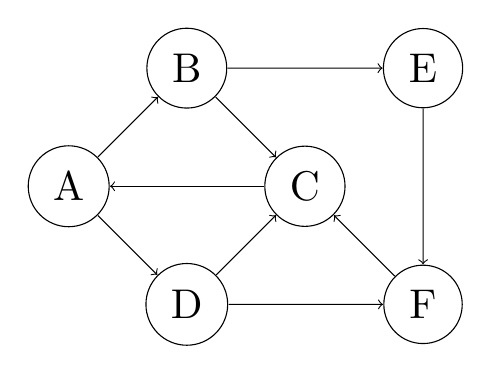
\begin{tikzpicture}[scale=1.5, transform shape]
        \node[draw, circle] (A) at (0,0) {A};
        \node[draw, circle] (B) at (1,1) {B};
        \node[draw, circle] (C) at (2,0) {C};
        \node[draw, circle] (D) at (1,-1) {D};
        \node[draw, circle] (E) at (3,1) {E};
        \node[draw, circle] (F) at (3,-1) {F};
        \draw[->] (A) -- (B);
        \draw[->] (A) -- (D);
        \draw[->] (B) -- (C);
        \draw[->] (B) -- (E);
        \draw[->] (D) -- (C);
        \draw[->] (D) -- (F);
        \draw[->] (C) -- (A);
        \draw[->] (E) -- (F);
        \draw[->] (F) -- (C);
    \end{tikzpicture}
    \caption{A Big Ball of Mud.}
    \label{fig:big_ball_of_mud}
\end{figure}

As we can see in Figure \ref{fig:big_ball_of_mud}, we do have circular dependencies and the code doesn't have any recognizable structure. If you have to create an object \code{C}, you'll have to instatiate almost the entire graph. This is a clear sign that the code is flawed.

If you work with such code, the goal must be to restructure the code such that the number of connections between the objects is minimized. In Figure \ref{fig:well_structured_code} is an example how this graph could look instead.

\begin{figure}[h]
    \centering
    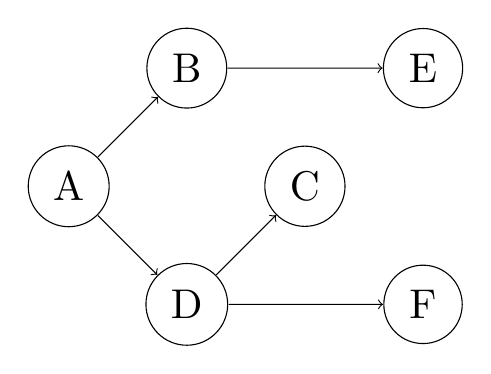
\begin{tikzpicture}[scale=1.5, transform shape]
        \node[draw, circle] (A) at (0,0) {A};
        \node[draw, circle] (B) at (1,1) {B};
        \node[draw, circle] (C) at (2,0) {C};
        \node[draw, circle] (D) at (1,-1) {D};
        \node[draw, circle] (E) at (3,1) {E};
        \node[draw, circle] (F) at (3,-1) {F};
        \draw[->] (A) -- (B);
        \draw[->] (A) -- (D);
        \draw[->] (B) -- (E);
        \draw[->] (D) -- (C);
        \draw[->] (D) -- (F);
    \end{tikzpicture}
    \caption{A well-structured code base represented as a tree.}
    \label{fig:well_structured_code}
\end{figure}

Here is a simple code example how you can break dependencies. Let's assume you have the following code:

\begin{programcode}{}   
\begin{verbatim}
# file_A.py
from enum import Enum

class A:
    class State(Enum):
        INIT = 0
        RUNNING = 1
        STOPPED = 2

    def do_something(self):
        return self.State.RUNNING

# file_B.py
def do_something_else():
    return A.State.RUNNING
\end{verbatim}
\end{programcode}

This code is bad because file\_B.py depends on the complete file\_A.py, even though it uses only a small fraction of its code. It would be better to move the State Enum to a separate file. This way file\_B.py doesn't have to depend on file\_A.py anymore. The code would look as follows:

\begin{programcode}{}
\begin{verbatim}
# file_enum.py
from enum import Enum
class State(Enum):
    INIT = 0
    RUNNING = 1
    STOPPED = 2 

# file_A.py
from file_enum import State

class A:
    def do_something(self):
        return State.RUNNING

# file_B.py
from file_enum import State

def do_something_else():
    return State.RUNNING

\end{verbatim}
\end{programcode}

There was no reason why the \code{State} enum should be within the \code{class A}. It was just a bad design decision. It might have made sense to put it there because the \code{class A} used it, but now the \code{class B} uses it as well. Therefore the \code{class B} has to import the entire \code{class A}.

If we instead move the \code{State} enum to a separate file, we can easily import it in both \code{class A} and \code{class B}. This way we have broken the dependency between the two files. The number of imports may not have been reduced, but the quality of the code has been significantly improved. Now the dependencies are cleaned up.

What we just did here is also known as the Interface Segragation Princeple (ISP). This principle states that you should have small interfaces because otherwise you import things that you don't need. And these things will clutter your code.

\section{Compilation Dependencies}

Many people adhere to the Dependency Inversion Principle (DIP)\footnote{TODO which book goes here?} by Robert C. Martin. This principle states that you should depend on abstractions (interfaces), not on concretions and one of the arguments is that it reduces compilation times. This is due to the fact that interfaces change way less often than implementations.

I'm not sure if this argument was ever true, but in most cases it is certainly wrong. The most obvious case are interpreted langauges where you don't have to compile your code at all. Therefore you don't gain anything by adding interfaces.

In C++ you define the interface of your classes in header files. The code using a certain class only includes the header files. Meanwhile you can change the implementation as much as you like, you'll only have to recompile the implementation files.

As far as I know, this is also the case in most other modern programming languages. I'm no Java expert, but as far as I could tell, Java didn't recompile the entire code base if you change a single implementation file. I don't know if this was due to a recent compiler optimization or if it was always like this. But one can certainly say that the DIP is outdated and one doesn't have to implement interfaces everywhere in order to keep the compilation times low.

It may have been the case in the early 2000s that one had to accompany every class with its own interface, but this is certainly not the case anymore. The compilation times are not detrimentally affected if you don't follow this principle. Only use interfaces if you want to use polymorphism. Everything else only clutters your code.

\section{Breaking Dependencies}

TODO do we need this section or should we split it up and move the explanations to the individual chapters?

TODO See p. 325-400

Breaking dependencies is probably the most important aspect of this book. This is due to the fact that dependencies make your code hard to test and that writing new code becomes pretty hard as well. 

Like the rest of this book, most techniques that I present are from Michael Feathrs book "Working Effectively with Legacy Code". The techniques are generally quite simple and the danger of introducing bugs is fairly low if applied correctly. However, there is always some risk involved, so you shouldn't apply these techniques lightly. For this reason I always explain the main difficulties of every technique.

I decided to explain these techniques in the chapters where they fit best. Here is a short overview of the techniques that I present in this book:

\begin{itemize}
    \item Excract Method, p. \pageref{sec:extract_method}
    \item The Dependency Injector, p. \pageref{sec:dependency_injection}
    \item TODO add all the techniques here
\end{itemize}

\subsection{Extract Method}\label{sec:extract_method}

It is very common that a class is too big. The class has too many methods and member variables. The class has too many responsibilities, it's a Big Ball of Mud. Everything depends on everything else. One thing you can do is to extract a method.

Let's assume we have the following code

\begin{programcode}{}
\begin{verbatim}
class Adder:
    def __init__(self):
        self.x = 5
        self.y = 3
        # ...

    def add(self):
        return self.x + self.y
    
    # ...

adder = Adder()
result = adder.add()
\end{verbatim}
\end{programcode}

The first thing we can do is defining a function \code{add\_new} which implements the functionality of the \code{add} method. In this example it's not really necessary, but in general it's a good idea to have a function that does the actual work and a class that manages the state. This way you can easily test the function \code{add\_new} without having to instatiate the class \code{Adder}. Now you can already write tests for the function without having to instantiate the whole class.

\begin{programcode}{}
\begin{verbatim}
def add_new(x, y):
    return x + y

class Adder:
    def __init__(self):
        self.x = 5
        self.y = 3
        # ...

    def add(self):
        return add_new(self.x, self.y)
    
    # ...

adder = Adder()
result = adder.add()
\end{verbatim}
\end{programcode}

As a second step, you can change all locations where the old \code{add} method was used. Then, you extract the complete method out of the class. Like this you can reduce its size. One drawback is that you somehow need access to the member variables of the class. For this reason you might have to make them public or at least write getter methods. This is an inevitable evil. You can't extract a method if you don't have access to the member variables.

However, once you're done with extracting methods and all the newly created functions are well tested, you should anyway restructure your class. You made so many changes that you can probably shrink the class and extract most of the variables into a separate data class (struct in C++).

\begin{programcode}{}
\begin{verbatim}
def add_new(x, y):
    return x + y

class Adder:
    def __init__(self):
        self.x = 5
        self.y = 3
        # ...
    
    # ...

adder = Adder()
result = add_new(adder.x, adder.y)
\end{verbatim}
\end{programcode}

The new function may have quite a lot of arguments. This should be refactored by creating some dataclasses (strcuts in C++) to group the arguments together. You can also extract several methods at once. By looking at the dependencies between the functions and the variables, you'll probably get an idea how you should structure the code.

In case you extracted all, or at least most methods that use x and y, you can extract also these variables and put them into a data class. This way you can reduce the size of the class even further.

\begin{programcode}{}
\begin{verbatim}
@dataclass
class AdderArguments:
    x: int
    y: int

def add_new(adder_arguments):
    return adder_arguments.x + adder_arguments.y

class Adder:
    def __init__(self):
        # ...
        pass
    
    # ...

adder_arguments = AdderArguments(5, 3)
result = add_new(adder_arguments)
\end{verbatim}
\end{programcode}

Admitedly, the usage of the \code{AdderArguments} is not really an improvement of the code here. I just introduced this dataclass to show you how you can group the arguments together. Generally, you should group the arguments together if may functions need the same arguments. 

\subsubsection*{Difficulties}

Extract Method is a fairly simple technique. You mainly have to pay attention that you don't mix up the function arguments. The old method probably had some arguments, plus all the member variables of the class that it used. So there may be quite a lot of arguments all together. In compiled languages you have the advantage that the compiler can warn you if you forgot some arguments or you mixed up the order. Especially if you work with default arguments, you have to be careful that you don't mix anything up.

Furthermore you have to make sure that you adapt all the method calls to the new function signature. Here the compiler can help you once you comment out or delete the old method.

\subsection{Extract Interface}


\section{Dependency Injection}\label{sec:dependency_injection}

Dependency Injection (DI), by Michael Feathers referred to as "parametrizing constructor", is a very common and powerful technique to pass functionality down the call stack. DI is particularly important if you have some object that you can't write unit tests for. This can be either because executing some method of this object is slow or it might not be deterministic, like communicating over a network connection.

Let's start with a small example. You have a file containing some numbers. You want to read this file and calculate the average of the numbers. The code could look like this:

\begin{programcode}{}\label{prog:average_of_file}
\begin{verbatim}
def average_of_file(file):
    with open(file, 'r') as f:
        contents = f.read()
    numbers = [int(x) for x in contents.split(',')]
    return sum(numbers)/len(numbers)

def test_read_file():
    assert average_of_file('test.csv') == 3
\end{verbatim} 
\end{programcode}

This code has two flaws. 

The first one is that it is potentially comparing floating point numbers for equality. But we'll neglect this issue for the time being.

The second flaw is that this isn't a unit test. It depends on the file system. This is bad because the file system is slow and it is not deterministic. The file might be deleted or the contents might change. This is why we have to use dependency injection. We have to pass the file contents to the function instead of reading it from the file system. Now the first step is that we have to take the code code appart. We split it into two functions, one function is responsible for calculating the average of the \code{numbers} and the other function is responsible for reading the file.

\begin{programcode}{}
\begin{verbatim}
def average_of_file(contents):
    numbers = [int(x) for x in contents.split(',')]
    return sum(numbers)/len(numbers)

def read_file():
    with open(file, 'r') as f:
        return f.read()

def test_read_file():
    assert average_of_file(read_file('test.csv')) == 3
\end{verbatim}
\end{programcode}

Now we can easily write a test which does not depend on the actual file. All we have to do is replacing the \code{read\_file} function with a mock that returns some random values.

\begin{programcode}{}
\begin{verbatim}
def average_of_file(contents):
    numbers = [int(x) for x in contents.split(',')]
    return sum(numbers)/len(numbers)

def read_mock(_):
    return '1,2,3,4,5'

def test_read_file():
    assert average_of_file(read_mock('test.csv')) == 3
\end{verbatim}
\end{programcode}

This is the basic idea of DI. But it's not yet the complete implementation. The \code{read\_mock} function may be burried within the code and it may be difficult to replace it. This is why we have to use a more sophisticated technique. We have to pass the function as an argument to \code{average\_of\_file}. This code looks as follows:

\begin{programcode}{}\label{prog:mock_reader}
\begin{verbatim}
def average_of_file(reader, file_name):
    numbers = file_reader(file_name)
    return sum(numbers)/len(numbers)

def mock_reader(_):
    return '1,2,3,4,5'

def file_reader(file_name):
    with open(file_name, 'r') as f:
        return f.read()

def test_read_file():
    assert average_of_file(mock_reader, 'test.csv') == 3
\end{verbatim}
\end{programcode}

We pass the code to read the file as a function argument to \code{average\_of\_file}. This is the basic idea of DI. You encapsulate the functionality into a function or a class and pass it on through the call stack. This way you can easily replace the functionality with a mock or a fake.

Note that DI is not limited to object-oriented (OO) code. You can also use it in procedural code as shown in the example above. The only requirement is that the programming language supports passing functions as arguments, which pretty much all programming langages do. For this reason, I won't make any difference between OO and procedural code in this book. The fundamental techniques required to refactor the code are exactly the same. In fact, writing OO code has its own set of problems. You have to deal with inheritance and classes which are too long, which can make the code even more complicated. We'll spend a fair amount of this book on problems that are specific to OO code.

Note that there are also mocking libraries avaiable to change the behavior of some functions being executed in your tests. Please don't use these libraries. They are a clear sign that your code is flawed. Use DI instead. It's really not that hard to pass a function as an argument to another function. Even if DI is currently not implemented in the code so far, adding it is usually not that hard.

\section{Fakes and Mocks}

As we have just seen, DI comes along with the usage of fakes and mocks. They both have in common that they replace functionality with some artificial result. The general idea behind fakes and mocks is that you want to replace some slow or unreliable functionality with a fast and deterministic object as it is required for unit tests.

Fakes and mocks are very similar as they have both the same goal. They are tools to replace some hard to test functionality with some artificial result.

Mocking is generally the easier thing to do. You just replace the object with a function that returns some predefined values as we have seen above. There's really not that much more left to explain.

Faking on the other hand can be much more difficult. In faking you replace a hard to test object with some artificial object that imitates at least some parts of the original object. A common example is creating a fake database or a file system. You implement a piece of code supporting a \code{read} and \code{write} function. The \code{write} function doesn't actually write to the DB or the file system. Instead, is just stores the corresponding values in the memory. Vice versa, when calling the \code{read} function, it doesn't actually read from the DB or the file system, but it returns the values stored in the memory. Like this you can mimic the behavior of the DB or the file system and write unit tests for your code.

\begin{programcode}{}
\begin{verbatim}
class FakeDB:
    def __init__(self):
        self.data = {}

    def write(self, key, value):
        self.data[key] = value

    def read(self, key):
        return self.data[key]
\end{verbatim}
\end{programcode}


In general I recommend writing mocks because they are so much simpler than fakes. You only need fakes if you really want to simulate some physical device.


\chapter{How to Test this Monstrosity}\label{chap:how_do_i_test_this_monstrosity}

Did I already mention that I'm not a big fan of OO code? I guess I did. And here is one of the reasons: classes can be difficult to instantiate. Especially if the constructor has some nasty side effects. If there are no default constructor available, you might have to instantiate a whole tree of objects just to test a single method. This is a clear sign that the code is flawed.

Now, of course, you can also have functions that are hard to deal with, but in general functions are easier to test than classes. You just pass the arguments and you get the result. This is not always the case with classes. This is one of the reasons why I prefer procedural code over OO code.

The most common issue with classes is that they have some side effects in the constructor. Most notably that they open a file, a network connection or it has some other side effects. This is a clear sign that the code is flawed. The constructor should only set the initial state of the object. It should not do anything else. You should be able to select this kind of functionality with DI. Whenever you deal with something that cannot be unit tested, you should use DI and here is one of the reasons why. If you incorporate such kind of behavior in the constructor, it may become impossible to unit test a whole blob of code.

And as I already said a few times, if you can't write unit tests, your code is bad. With that respect, this chapter here is not only about unit testing, it also contains valueable information if you want to improve the quality of your code.

There are a few problems we can encounter that make working with a class difficult:
\begin{itemize}
    \item The constructor has no default constructor.
    \item The constructor does excessive amount of work.
    \item The constructor has side effects.
    \item You don't know what arguments you have to pass to the constructor.
\end{itemize}

I hope you see why I don't like OO programming. There's just too much that can go wrong that makes your code untestable. Here we see why you should never write any complex code in the constructor. It makes the code untestable. Unfortunately, many programmers don't know about this issue and they write all kinds of functionality into the constructor.

Now we want to look at a few techniques to circumvent these issues.

\section{Just Instatiate the Class}

How do you deal with code that contains a excessively complicated constructor?

The best attempt is probably to wirte the unit test nevertheless. And once you run or compile the test, you will see where it actually breaks. Maybe you don't need to construct the entire class instance tree because it's not used by your unit test. If this is the case, lucky you. This is one of the cases where working in an interpreted language has some advantages because you might not need the entire object tree to run the test. You might need only a subset of the objects. Contrary to compiled languages where you have to instantiate the entire object tree. Or at least mock or fake the objects that you don't need.

However, if your test somehow miraculously passes, you have to make sure that it really tests what you think it does. In order to do this, you have to deliberately break the code and see if it fails. If it doesn't fail, there is something terribly wrong with your test. This technique is generally recommended if you do anything else than TDD (p. \pageref{chap:tdd}). Because otherwise you never know what your test actually tests.

If you are programming in a compiled language, you have to make sure that all the objects instantiated support the corresponding functions. If you don't know what value you should instantiate these objects with, try something like \code{Null}, \code{nullptr} or similar, depending on the programming language you work with.

\section{The Dependency Injectior}\label{sec:dependency_injector}

Once the test runs, you have to make sure that it fulfills the criteria of a unit test. This means that the test has to be fast and deterministic. It shouldn't depend on things like a network connection, a database or the file system. These things all have to be faked or mocked away.

As we have already seen, DI is the remedy of choice for such issues. And there is absolutely nothing wrong about implementing DI in your code. In fact, it is quite simple. In interpreted languages it is very simple to get it running. In compiled languages it takes somewhat more efforts because you have to implement an interface for the existing code. And if you can't replace the existing code, you'll have to write a wrapper around it. This is a bit more work, but it is still feasible. 

\subsection{Writing Tests with the Dependency Injector}

Once you used the dependency injector, it is fairly simple to write tests. At least from a technical point of view. As I'll explain below, you just have to make them run (in interpreted langauges) or compile (in comipled languages). The difficult question is rather: are the tests correct?

For both, interpreted and compiled languages, you can simply start implementing the corresponding mock or fake and use it in your tests. In interpreted languages the tests will run as soon as you implemented all the methods used. In compiled languages, the code will compile once you have implemented all the methods of the interface. In both cases, the interpreter or the compiler will tell you if you forgot something. So it's a fairly fail-safe method. Michael Feathers calls this process "Extract Interface".

The most common problem is that you don't know if you can mock something or if this is going to affect the final result of the test. The simplest way to find out is that you just write the tests and see what happens. This is very similar to TDD. You write all kinds of tests and if they all pass, the code is most likely fine. Of course, this technique has some pitfalls as well. Most notably, you'll have to know what the code does. You have to be able to write test upfront. If you are not sure what the code does, you're in trouble. But this is a very general problem. You have to know what the code does in order to write tests for it. Otherwise you'll never know if your tests are correct. You can still use the dependency injector, you just don't know if the tests using fakes are correct.

There are two ways to solve this issue and they both start the same way: you run the code and use the debugger to keep track of all the variables. Then you can either write tests using the values of these variables and mock the objects accordingly. Or you write your tests on a higher level.


\subsection{Interpreted Languages}

As we've already seen, for interpreted languages implementing DI is really simple. This is due to the duck typing, which allows you to pass any object that supports the same functions, opposite to compiled languages where you have to define an interface or an abstract base class to use polymorphism. Let's take a look again at the example on p. \pageref{prog:average_of_file}.

\begin{programcode}{}
\begin{verbatim}
def average_of_file(file_name):
    with open(file_name, 'r') as f:
        contents = f.read()
    numbers = [int(x) for x in contents.split(',')]
    return sum(numbers)/len(numbers)

if __name__ == '__main__':
    print(average_of_file('test.csv'))
\end{verbatim}
\end{programcode}

Now we can take the code that we don't like and put it into a dedicated function. Then we pass the function as a function argument. At the same time, we can also implement a fake function that returns some predefined values. This code looks as follows:

\begin{programcode}{}
\begin{verbatim}
def read_file(file_name):
    with open(file_name, 'r') as f:
        return f.read()

def fake_file(_):
    return '1,2,3,4,5'

def average_of_file(file_name, reader=read_file):
    contets = reader(file_name)
    numbers = [int(x) for x in contents.split(',')]
    return sum(numbers)/len(numbers)

print(average_of_file('test.csv'))
print(average_of_file('not_existing.txt', fake_file))
\end{verbatim}
\end{programcode}

That's it, you're done. Now you can write unit tests that use the \code{fake\_file} function.

It is important to mention that the default argument should be the object that was used so far. This way you don't have to change the existing code and the chances of breaking something are minimized.

If you decide not to use default arguments for whatever reason, you'll have to change all the function calls in the code. This can be tedious in a very large code base. I recommend to use default arguments, unless you work with some programming language that doesn't support them.

\subsection{Compiled Languages}

In compiled languages, we have to distinguish between DI for functions or classes. For functions, the process is quite similar to the one in interpreted languages. You just have to pass the function as an argument to the other function. You can just implement a mock function and pass it as a function argument. 

For classes, the process is a bit more complicated. You have to implement an interface for the existing code. In C++, you have to pass a pointer to the base class. This is especially cumbersome if the class is from a third party API. In this case you cannot change the class. Instead, you have to write a wrapper around the class and implement the code using the wrapper.

\begin{programcode}{}
\begin{verbatim}
#include <filesystem>
#include <ifstream>
#include <iostream>

using namespace std; 

class FileReader{
public:
    string print_lines(const string& file_name){
        ifstream file(filename);
        string line;
        while (getline(file, line)) {
            cout << line << endl;
        }
    }
};

int main() {
    RealFileReader reader;
    reader.print_lines("some_file.txt");
}
\end{verbatim}
\end{programcode}

Now there are two cases: either we have access to the source code of the \code{FileReader} class and we can make it inherit from a base class, or we don't have access to the source code and we have to write a wrapper around it. In the first case, the code looks as follows:


\begin{programcode}{}
\begin{verbatim}
#include <ifstream>
#include <iostream>

using namespace std; 

class FileReader{
public:
    string print_lines(const string& file_name) = 0;
};

class RealFileReader : public FileReader{
public:
    string print_lines(const string& file_name) override {
        ifstream file(filename);
        string line;
        while (getline(file, line)) {
            cout << line << endl;
        }
    }
};

class FakeFileReader : public FileReader{
public:
    string print_lines(const string&) override {
        cout << "line 1" << endl;
        cout << "line 2" << endl;
    }
};

int main() {
    auto reader = make_unique<RealFileReader>();
    reader->print_lines("some_file.txt");
}
\end{verbatim}
\end{programcode}

This took some efforts as we are working with C++ afterall. But it is still feasible. The other case is when we don't have access to the source code of the \code{FileReader} class. In this case we have to write a wrapper around it. This code looks as follows:

\begin{programcode}{}
\begin{verbatim}
#include <ifstream>
#include <iostream>

using namespace std;

class FileReaderWrapperBase{
public:
    string print_lines(const string& file_name) = 0;
};

class RealFileReaderWrapper : public FileReaderWrapperBase{
public:
    string print_lines(const string& file_name){
        FileReader reader;
        reader.print_lines(file_name);
    }
};

class FakeFileReaderWrapper : public FileReaderWrapperBase{
public:
    string print_lines(const string& file_name){
        cout << "line 1" << endl;
        cout << "line 2" << endl;
    }
};

int main() {
    auto reader = make_unique<RealFileReaderWrapper>();
    reader->print_lines("some_file.txt");
}
\end{verbatim}
\end{programcode}

Yes, this is the technique to mock a class in C++ if you don't have access to it. The efforts required are moderate since you only have to wrap the methods that you really need. You just have to know this trick and you have no more excuses not to use DI.

\subsection{Not Instantiable Arguments}

When working with legacy code, you may struggle to instantiate some objects that you need for your tests. This problem may show up regardless whether you work with functions, methods or classes. The reasons can be manifold but they are always a sign for bad code. As we learned, good code is easy to test. And if it's not easy to test, it is most likely bad. 

The solution is always the same, regardless if you work with functions, methods or classes. You should use the dependency injector (p. \pageref{sec:dependency_injector}). This is the gold standard. The dependency injector allows you to fake or mock the object which is hard to instantiate or has side effects. You are not going to test these objects that are hard to instantiate anyway because you can't. You'd have to fix them, but that's another story. Instead you want to test the code that uses these objects. You want to test everything else.

\begin{programcode}{}
\begin{verbatim}
class A:
    def __init__(self):
        # assume we have some bad side effects here
        pass

    def return_A(self):
        return "A"
    
class B:
    def return_B(self):
        return "B"

def my_function(a, b):
    return a.return_A() + b.return_B()

# in tests.py
def test_my_function_returns_A():
    assert my_function(A(), B()) == "AB"
\end{verbatim}
\end{programcode}

This would be perfectly viable code, if it wasn't for the bad side effect in the constructor of \code{A}. Now what we have to do instead is to apply the dependency injector and create a mock for \code{A}. As we are using Python, we don't need a base class. It is sufficient to write a class that implements the same methods as \code{A}.

\begin{programcode}{}
\begin{verbatim}
class mock_A:
    def return_A(self):
        return "A"

class A:
    def __init__(self):
        # assume we have some bad side effects here
        pass

    def return_A(self):
        return "A"
   
class B:
    def return_B(self):
        return "B"

def my_function(a, b):
    return a.return_A() + b.return_B()

# in tests.py
def test_my_function_returns_A():
    assert my_function(mock_A(), B()) == "AB"
\end{verbatim}
\end{programcode}

Like this we no longer have to call the bad constructor of \code{A}, but we can use the mock instead. Now, the test doesn't test the functionality of \code{A} any longer. But this wasn't the idea of this test anyway. The idea was to test the interplay of \code{A} and \code{B} in the function \code{my\_function}. The class \code{A} will have to be dismanteled and tested independently.


\subsection{Costructor with Side Effects}

Let's say you have the following code with a counter implemented inside the constructor. This might have seemed like a reasonable thing to do, but now as you start writing unit tests, you realize that this has severe drawbacks.

\begin{programcode}{}
\begin{verbatim}
class Counter:
    counter = 0

    def __init__(self):
        Counter.counter += 1

    def get_counter(self):
        return Counter.counter

if __name__ == '__main__':
    counter = Counter()
    print(counter.get_counter()) # prints 1
    counter2 = Counter()
    print(counter2.get_counter()) # prints 2
\end{verbatim}
\end{programcode}

At first, this may not seem like a problem. Only once you wrote a few tests, you realize the drawbacks of this design.

\begin{programcode}{}
\begin{verbatim}
def test_counter1():
    counter = Counter()
    assert counter.get_counter() == 1

def test_counter2():
    counter = Counter()
    assert counter.get_counter() == 2
\end{verbatim}
\end{programcode}

Now it might dawn on you that you have a problem. The tests are locked. If you swap them, they fail. They depend on external factors (the \code{counter}) which is a no-go for unit tests.

Unfortunately there is no single rule how to deal with this issue. Each and every case needs to be looked at individually. But there are a few common techniques that you can use to deal with this issue.

\subsection{Remove the Side Effects}

This is of course the gold standard. If you can get rid of the side effects in the constructor, you should do so. However, this is usually not possible. There might be a reason why the constructor looks the way it does.

\subsection{Undo the Side Effects in the Destructor}

This is generally already more feasible than removing the side effects completely. If you undo them in the Destructor, you destroy the object and the side effects are gone. This works at times. For example if you open a file inside the constructor, you may want to close it in the destructor. Though, of course, this doesn't always work. The idea of the counter mentioned above is to keep the state.

\subsection{Undo the Side Effects in a Separate Function}

Now here things get a little ugly. If the solutions mentioned above don't work, you'll have to take some desperate measures. You have to introduce code that is only dedicated for testing purposes. This is a very bad sign. You should never have to write production code for testing purposes. This is the tail wagging the dog. This is a desperate measure that you should avoid at all costs. But you work with legacy code and sometimes there is no other way to get the code under test. So let's see how this code could look like.

Inside the class \code{Counter} we add a new function \code{set\_counter} that allows us to set the counter to any value we want. This function is only used for testing purposes. Note that the user code doesn't change at all.

\begin{programcode}{}
\begin{verbatim}
class Counter:
    counter = 0

    def __init__(self):
        Counter.counter += 1

    def get_counter(self):
        return Counter.counter

    def set_counter(self, value):
        Counter.counter = values

if __name__ == '__main__':
    counter = Counter()
    print(counter.get_counter()) # prints 1
    counter2 = Counter()
    print(counter2.get_counter()) # prints 2
\end{verbatim}
\end{programcode}

In the test code we now have to set the counter for every test case. This is the only way to make the code testable.

\begin{programcode}{}
\begin{verbatim}
def test_counter1():
    counter = Counter()
    counter.set_counter(1)
    assert counter.get_counter() == 1

def test_counter2():
    counter = Counter()
    counter.set_counter(1)
    assert counter.get_counter() == 1
\end{verbatim}
\end{programcode}

As I said, this is an ugly hack. But it's the only solution that I know.

TODO: reread the chapter on testing classes and see if there is something that can be added here.

\section{Nested Constructor Arguments}

DI is not always easily applicable. Especially if you have a class that is instantiated deep within a constructor. Needless to say that this is a clear sign of bad code. But we are dealing with legacy code and we have to make the best of it.

\begin{programcode}{}
\begin{verbatim}
class Car:
    def __init__(tires, pistons):
        self.tires = tires
        fuel_pump = FuelPump()
        # ...
        self.engine = Engine(pistons, fuel_pump)
\end{verbatim}
\end{programcode}

Now the problem is very obvious. It is difficult to instantiate the \code{engine} using DI because it is hard to extract.

\begin{programcode}{}
\begin{verbatim}
class Car:
    def __init__(tires, piston):
        self.tires = tires
        fuel_pump = FuelPump()
        # ...
        self.engine = Engine(piston, fuel_pump)

    def supersede_engine(self, new_engine):
        self.engine = new_engine
\end{verbatim}
\end{programcode}

In Python and other languages with a grabage collector, this is a fairly simple thing to do. However in older languages such as C++, you might run into memory issues. In these programming languages, you have to make sure that you don't create a memory leak. This isn't a problem if you use smart pointers, but I assume if you read this book, that you might work with legacy code that uses raw pointers. In this case, you'll have to use the \code{delete} keyword to free the memory.

\begin{programcode}{}
\begin{verbatim}
def test_car():
    tires = ...
    car = Car(tires, piston)

    car.supersede_engine(MockEngine())
    car.drive(50)

    assert car.engine.rpm == 1000
\end{verbatim}
\end{programcode}

Now this code is strictly inferior to the code using DI because your test code is different than your production code. This is always a sign that your code is flawed and the reason is that your constructor does too much. But as always, you work with legacy code and you might not have any other choice than superseding some variables.

\section{Singletons}

Singletons are one of the worst antipatterns in software engineering. Singletons might have a few applications, but in general it is much better to avoid it at all costs. Is only leads to bad code. And if you don't believe me, try writing some unit tests and you'll probably face some serious issues because the tests may depend on each other. This is a clear no-go in unit testing. All tests should be independent of each other.

Let's make a very small example.

\begin{programcode}{}
\begin{verbatim}
def get_data_form_db():
    db_connector = DBConnector()
    return db_connector.get_data()
\end{verbatim}
\end{programcode}

Here, \code{DBConnector} is a singleton. This code is bad for two reasons. The first one we learned in the section on DI and unit testing. The \code{DBConnector} connects to a database and therefore this code cannot be unittested.

Furthermore, this is a singleton and if it has some form of internal state, it will behave differently each time you call it.

The solution is the same as always: DI. You should pass the \code{DBConnector} as an argument to the function. This way you can easily replace the \code{DBConnector} with a mock or a fake.

\begin{programcode}{}
\begin{verbatim}
def get_data_form_db(db_connector=DBConnector()):
    return db_connector.get_data()
\end{verbatim}
\end{programcode}

And the test code will look as follows:

\begin{programcode}{}
\begin{verbatim}
def test_get_data_form_db():
    db_connector = MockDBConnector()
    assert get_data_form_db(db_connector) == "some data"
\end{verbatim}
\end{programcode}

In my opinion it would be even better to create a \code{db\_connetion} object in the \code{main} function or at least in some location where it is call very few times and then pass it as a function argument to the functions that actually need access to the database. Like this you never need a singleton. The only drawback is that you have to pass an additional argument through the function stack. But for well written code, there are not so many functions that need this argument and otherwise you can create a dataclass that contains all the information needed for the database connection, logging, etc. This allows you to keep the number of arguments low.

\section{Global Variables}



\section{I Can't Test this Method}

Similar to clases, there can be problems if you want to test a method or function:

\begin{itemize}
\item The method is private
\item The method has side effects
\item You don't know how to instantiate the arguments
\end{itemize}

\subsection{The Method is Private}

If you feel like testing a method which is private, just make it public. This is certainly not recommended for good code, but here we are dealing with legacy code. And getting the method under test is more important.

Once you made the method public, you can write unit tests for it. And when you have plenty of unit tests, you might be able to extract this method, maybe along with some other methods, into a new class or a set of freestanding functions. The fact that you wanted to test this method to begin with is a clear indication that it is too complicated and should be refactored. So, alltogether, refactoring this method into its own class is anyway a good idea.

Once you have the method tested, use extract method to make the method a free standing function. If required, you can then incorporate the method into a new class.

Let's make a small example. Assume that we have the class \code{A} with a private method \code{do\_something} that contains very complicated code and we're feeling a strong urge to test it.

\begin{programcode}{}
\begin{verbatim}
class A{
private:
    int b = 1;
    void do_something(){
        // some very complicated code
        std::cout << b << std::endl;
    }
public:
    void do_something_public(){
        do_something();
    }
};
\end{verbatim}
\end{programcode}

The first step is very simple. We just make the method public.

\begin{programcode}{}
\begin{verbatim}
class A{
private:
    int b = 1;
public:
    void do_something(){
        // some very complicated code
        std::cout << b << std::endl;
    }
    void do_something_public(){
        do_something();
    }
};
\end{verbatim}
\end{programcode}

The next step is to write a unit test for the method. This may be laborious, depending on the code. In case you face some difficulties, look up the techniques in the chapter "How Do I Test this Monstrosity" (p. \pageref{chap:how_do_i_test_this_monstrosity}).

Once you have the tests in place, you can extract method (p. \pageref{sec:extract_method}) and make the method a free standing function. If required, you can then incorporate the method into a new class.

\subsubsection*{Final}

Making methods \code{final} or \code{sealed} is generally a good thing. In fact, this should be the standard and overriding functions should only be allowed if it is explicitly allowed. With that respect, many OO programming languages are flawed. There were times when it was considered good practice if a test case inherits from the class it is testing. But this is a really bad idea. This is similar to testing private (or protected) methods. You should always test the public interface of a class. Never the private methods. You should only test private methods if you are working with legacy code.

In my opinion you should never write tests that inherit from the class under test. The worst thing you have to do is making private methods public and then refactor the code once it's tested.

\subsubsection*{The Method has Side Effects}

First, let's think about good code. In good code, all the changes that a method or function makes are immediately visible to the outside. These functions only depend on the function arguments and the only thing they do is calculating the return value. They are called pure functions and are the gold standard of good code. In fact, functional programming is all about writing pure functions.

Unfortunately, once in a while you have to communicate to the outside. Either by reading a file, writing to a database or sending a message over the network. This is when you have to deal with side effects. And this is when you have to deal with the problem of testing these functions.

But you can limit these side effects to a minimum. Robert C. Martin calls this a humble object. It has only one job: get the data from a file and return it. You won't be able to write a unit test for this function, but the function is so simple that it shouldn't be necessary.

Our goal is to wirte as many pure functions as possible and limit the side effects to a minimum. This makes the code easier to test and easier to understand.

Now you might already see one problem with pure functions: methods are generally not pure functions. They frequently have side effects as they change the member variables of the class. This is the main reason why I don't like classes. Classes have hidden states and are therefore hard to understand and hard to test.

A common example is the following code that we've already seen on p. \pageref{prog:average_of_file}.

\begin{programcode}{}\label{prog:mock_reader}
\begin{verbatim}
def average_of_file(reader, file_name):
    numbers = file_reader(file_name)
    return sum(numbers)/len(numbers)

def mock_reader(_):
    return '1,2,3,4,5'

def file_reader(file_name):
    with open(file_name, 'r') as f:
        return f.read()

def test_read_file():
    assert average_of_file(mock_reader, 'test.csv') == 3
\end{verbatim}
\end{programcode}

Here the function \code{file\_reader} has a side effect. It reads from the file system. This is what Robert C. Martin called a humble object. We stirpped down this function to the bare minimum and made it as simple as possible. We will not be able to write a unit test for this function, but it is so simple that it shouldn't be necessary. For the unit tests we can use a mock function that returns some predefined values.

\section{The sensing Variable}

There are times when you have to deal with a very complicated function and you don't know how to get it under test. One option to deal with such functions it to use a sensing variable which helps you to keep track of the code. The sensing variable is not used in the production code, it is only there for testing purposes.

Let's have a look at this code. It is hard to write tests for it and you don't really know what it is all about. But you know that under certain conditions, the function \code{do\_something} is getting executed. But how do you test this?

\begin{programcode}{}
\begin{verbatim}
def some_complicated_function(a, b, c):

    # ...
    if a > 1:
        if b < 10:
            do_something(a)
    # ...
\end{verbatim}
\end{programcode}

What you can do is to introduce a sensing variable. You introduce an artificial boolean whose only task is to keep track if the function \code{do\_something} was executed. This is how the code looks like:

\begin{programcode}{}
\begin{verbatim}
def some_complicated_function(a, b, c):
    do_something_executed = False
    # ...
    if a > 1:
        if b < 10:
            do_something(a)
            do_something_executed = True
    # ...
    return do_something_executed
\end{verbatim}
\end{programcode}

The variable \code{do\_something\_executed} is only \code{True} if the function \newline \code{do\_something} was executed. So you can use the return value of the function to check if the function was executed. This is a very simple technique that can help you to keep track of the code. It is not a perfect solution, but it is better than nothing.

\section{What Methods Should I Test?}

This is another difficult topic. As the code may have side effects and use global variables, in theory you have to check all the code that could be affected by the change. You'd have to test everything. In the extreme case you'd have to test almost the entire code base. For very bad code, this is indeed the only option you have: write integration tests that cover all the code but are slow and impresice. You won't get such a good feedback as you could when writing unit tests, but it's better than nothing.

Now a general thing that you can do is using DI (p. \pageref{sec:dependency_injection}). DI is your friend because it helps you to get these dependencies under control. Just mock or fake a method and your code becomes much simpler to understand. Once you mocked the most complicated methods, your code should be easy to understand and therfore also easy to test.

The algorithm to deal with such methods or functions is as follows:
\begin{enumerate}
    \item Write a few tests for any interface you can find. This can also be the input and output of the entire software. I just hope that your software has some kind of interface.
    \item Implement DI. Use the tests to see if the code still works.
    \item Write a mock for the method that you implemented DI for.
    \item Write unit tests for the method.
    \item Change the method.
\end{enumerate}


\begin{programcode}{}
\begin{verbatim}
def file_reader(file_name):
    with open(file_name, 'r') as f:
        return f.read()

def average_of_file(reader, file_name):
    contents = reader(file_name)
    numbers = [int(x) for x in contents.split(',')]
    return sum(numbers)/len(numbers)

if __name__ == '__main__':
    print(average_of_file(file_reader, 'test.csv'))
\end{verbatim}
\end{programcode}


\begin{programcode}{}
\begin{verbatim}
def mock_reader(_):
    return '1,2,3,4,5'

def average_of_file(reader, file_name):
    contents = reader(file_name)
    numbers = [int(x) for x in contents.split(',')]
    return sum(numbers)/len(numbers)

def test_average_of_file():
    assert average_of_file(mock_reader, 'test.csv') == 3
\end{verbatim}
\end{programcode}
 
\chapter{Conclusions}

Working with legacy code is a real pain. The real issue is not that it's hard to change, but rather that you don't know what the code does. You never know if the code is in the correct state just by looking at it. This is a real issue because if you ever have a bug in your code, you don't know where this faulty behavior occured. You randomly have to choose some point in your code and fix the behavior with an \code{if} statement, making the code even worse.

Michael Feathers gave us the vocabluary and techniques required to work with legacy code. As he wrote several times, you need to test your code using unit tests. The most commonly used steps to improve achieve this goal are:
\begin{enumerate}
    \item Instantiate a class in a unit test.
    \item If it doesn't work, use the dependency injector.
    \item Mock or fake the object you can now inject.
    \item Lean on the compiler or interpreter until you implemented all methods needed.
    \item Write unit tests for the methods.
\end{enumerate}




\backmatter%%%%%%%%%%%%%%%%%%%%%%%%%%%%%%%%%%%%%%%%%%%%%%%%%%%%%%%
%\include{glossary}
%\include{solutions}
\printindex

%%%%%%%%%%%%%%%%%%%%%%%%%%%%%%%%%%%%%%%%%%%%%%%%%%%%%%%%%%%%%%%%%%%%%%

\end{document}





